% Options for packages loaded elsewhere
\PassOptionsToPackage{unicode}{hyperref}
\PassOptionsToPackage{hyphens}{url}
\PassOptionsToPackage{dvipsnames,svgnames,x11names}{xcolor}
%
\documentclass[
  11pt,
  letterpaper,
]{article}

\usepackage{amsmath,amssymb}
\usepackage{iftex}
\ifPDFTeX
  \usepackage[T1]{fontenc}
  \usepackage[utf8]{inputenc}
  \usepackage{textcomp} % provide euro and other symbols
\else % if luatex or xetex
  \usepackage{unicode-math}
  \defaultfontfeatures{Scale=MatchLowercase}
  \defaultfontfeatures[\rmfamily]{Ligatures=TeX,Scale=1}
\fi
\usepackage{lmodern}
\ifPDFTeX\else  
    % xetex/luatex font selection
\fi
% Use upquote if available, for straight quotes in verbatim environments
\IfFileExists{upquote.sty}{\usepackage{upquote}}{}
\IfFileExists{microtype.sty}{% use microtype if available
  \usepackage[]{microtype}
  \UseMicrotypeSet[protrusion]{basicmath} % disable protrusion for tt fonts
}{}
\makeatletter
\@ifundefined{KOMAClassName}{% if non-KOMA class
  \IfFileExists{parskip.sty}{%
    \usepackage{parskip}
  }{% else
    \setlength{\parindent}{0pt}
    \setlength{\parskip}{6pt plus 2pt minus 1pt}}
}{% if KOMA class
  \KOMAoptions{parskip=half}}
\makeatother
\usepackage{xcolor}
\usepackage[margin=1in]{geometry}
\setlength{\emergencystretch}{3em} % prevent overfull lines
\setcounter{secnumdepth}{-\maxdimen} % remove section numbering
% Make \paragraph and \subparagraph free-standing
\ifx\paragraph\undefined\else
  \let\oldparagraph\paragraph
  \renewcommand{\paragraph}[1]{\oldparagraph{#1}\mbox{}}
\fi
\ifx\subparagraph\undefined\else
  \let\oldsubparagraph\subparagraph
  \renewcommand{\subparagraph}[1]{\oldsubparagraph{#1}\mbox{}}
\fi


\providecommand{\tightlist}{%
  \setlength{\itemsep}{0pt}\setlength{\parskip}{0pt}}\usepackage{longtable,booktabs,array}
\usepackage{calc} % for calculating minipage widths
% Correct order of tables after \paragraph or \subparagraph
\usepackage{etoolbox}
\makeatletter
\patchcmd\longtable{\par}{\if@noskipsec\mbox{}\fi\par}{}{}
\makeatother
% Allow footnotes in longtable head/foot
\IfFileExists{footnotehyper.sty}{\usepackage{footnotehyper}}{\usepackage{footnote}}
\makesavenoteenv{longtable}
\usepackage{graphicx}
\makeatletter
\def\maxwidth{\ifdim\Gin@nat@width>\linewidth\linewidth\else\Gin@nat@width\fi}
\def\maxheight{\ifdim\Gin@nat@height>\textheight\textheight\else\Gin@nat@height\fi}
\makeatother
% Scale images if necessary, so that they will not overflow the page
% margins by default, and it is still possible to overwrite the defaults
% using explicit options in \includegraphics[width, height, ...]{}
\setkeys{Gin}{width=\maxwidth,height=\maxheight,keepaspectratio}
% Set default figure placement to htbp
\makeatletter
\def\fps@figure{htbp}
\makeatother
\newlength{\cslhangindent}
\setlength{\cslhangindent}{1.5em}
\newlength{\csllabelwidth}
\setlength{\csllabelwidth}{3em}
\newlength{\cslentryspacingunit} % times entry-spacing
\setlength{\cslentryspacingunit}{\parskip}
\newenvironment{CSLReferences}[2] % #1 hanging-ident, #2 entry spacing
 {% don't indent paragraphs
  \setlength{\parindent}{0pt}
  % turn on hanging indent if param 1 is 1
  \ifodd #1
  \let\oldpar\par
  \def\par{\hangindent=\cslhangindent\oldpar}
  \fi
  % set entry spacing
  \setlength{\parskip}{#2\cslentryspacingunit}
 }%
 {}
\usepackage{calc}
\newcommand{\CSLBlock}[1]{#1\hfill\break}
\newcommand{\CSLLeftMargin}[1]{\parbox[t]{\csllabelwidth}{#1}}
\newcommand{\CSLRightInline}[1]{\parbox[t]{\linewidth - \csllabelwidth}{#1}\break}
\newcommand{\CSLIndent}[1]{\hspace{\cslhangindent}#1}

\usepackage{amsfonts}
\DeclareMathAlphabet{\mathams}{U}{msb}{m}{n}
\usepackage{algorithm}
\usepackage{algpseudocode}
\usepackage{booktabs}
\usepackage{longtable}
\usepackage{array}
\usepackage{multirow}
\usepackage{wrapfig}
\usepackage{float}
\usepackage{colortbl}
\usepackage{pdflscape}
\usepackage{tabu}
\usepackage{threeparttable}
\usepackage{threeparttablex}
\usepackage[normalem]{ulem}
\usepackage{makecell}
\usepackage{xcolor}
\makeatletter
\makeatother
\makeatletter
\makeatother
\makeatletter
\@ifpackageloaded{caption}{}{\usepackage{caption}}
\AtBeginDocument{%
\ifdefined\contentsname
  \renewcommand*\contentsname{Table of contents}
\else
  \newcommand\contentsname{Table of contents}
\fi
\ifdefined\listfigurename
  \renewcommand*\listfigurename{List of Figures}
\else
  \newcommand\listfigurename{List of Figures}
\fi
\ifdefined\listtablename
  \renewcommand*\listtablename{List of Tables}
\else
  \newcommand\listtablename{List of Tables}
\fi
\ifdefined\figurename
  \renewcommand*\figurename{Figure}
\else
  \newcommand\figurename{Figure}
\fi
\ifdefined\tablename
  \renewcommand*\tablename{Table}
\else
  \newcommand\tablename{Table}
\fi
}
\@ifpackageloaded{float}{}{\usepackage{float}}
\floatstyle{ruled}
\@ifundefined{c@chapter}{\newfloat{codelisting}{h}{lop}}{\newfloat{codelisting}{h}{lop}[chapter]}
\floatname{codelisting}{Listing}
\newcommand*\listoflistings{\listof{codelisting}{List of Listings}}
\makeatother
\makeatletter
\@ifpackageloaded{caption}{}{\usepackage{caption}}
\@ifpackageloaded{subcaption}{}{\usepackage{subcaption}}
\makeatother
\makeatletter
\@ifpackageloaded{tcolorbox}{}{\usepackage[skins,breakable]{tcolorbox}}
\makeatother
\makeatletter
\@ifundefined{shadecolor}{\definecolor{shadecolor}{rgb}{.97, .97, .97}}
\makeatother
\makeatletter
\makeatother
\makeatletter
\makeatother
\ifLuaTeX
  \usepackage{selnolig}  % disable illegal ligatures
\fi
\IfFileExists{bookmark.sty}{\usepackage{bookmark}}{\usepackage{hyperref}}
\IfFileExists{xurl.sty}{\usepackage{xurl}}{} % add URL line breaks if available
\urlstyle{same} % disable monospaced font for URLs
\hypersetup{
  pdftitle={Qualifying Exam},
  pdfauthor={Art Tay},
  colorlinks=true,
  linkcolor={blue},
  filecolor={Maroon},
  citecolor={Blue},
  urlcolor={Blue},
  pdfcreator={LaTeX via pandoc}}

\title{Qualifying Exam}
\author{Art Tay}
\date{}

\begin{document}
\maketitle
\ifdefined\Shaded\renewenvironment{Shaded}{\begin{tcolorbox}[interior hidden, borderline west={3pt}{0pt}{shadecolor}, boxrule=0pt, breakable, enhanced, frame hidden, sharp corners]}{\end{tcolorbox}}\fi

\hypertarget{introduction}{%
\section{Introduction}\label{introduction}}

\begin{itemize}
\item
  Overview of the problem area.

  \begin{itemize}
  \tightlist
  \item
    Graphs are an important data structure.

    \begin{itemize}
    \tightlist
    \item
      GRAPHS provide an incredibly flexible structure for modeling
      complex data. Data can naturally appear as graphs, like molecules.
      We can reduce data to a graph, such as the key points of a image.
      We can even use graphs to add structure, such as grammatical
      relationships.
    \end{itemize}
  \item
    GNN models are good at prediction and inference on graph data.

    \begin{itemize}
    \tightlist
    \item
      Graph Neural Networks (GNNs) have become a popular choice for
      prediction and inference on graph data. At their core, GNNs work
      by iteratively updating node embeddings based on information from
      neighboring nodes. The idea is to use the graph's structure to
      engineer better features. This message passing scheme allows GNNs
      to capture complex dependencies and patterns present within the
      graph structure. GNN architectures typically consist of multiple
      layers, each performing message passing and aggregation operations
      to refine the embeddings. These layers are often followed by
      pooling and dense prediction layers to produce the final output.
    \end{itemize}
  \item
    There are many important applications for graph classification
    models.

    \begin{itemize}
    \tightlist
    \item
      Some important applications of graph classification include
      predicting chemical toxicity (Bai et al. 2019), classifying
      proteins (Gallicchio and Micheli 2019), and even detecting cancer
      from pathology slides (Xiao et al. 2023).
    \end{itemize}
  \item
    \textbf{Problem:} While GNNs achieve remarkable predictive power,
    their complexity prevents the exaction of the scientific rationale.
  \end{itemize}
\item
  Why is the problem important?

  \begin{itemize}
  \tightlist
  \item
    Explaining or interpreting GNN predictions would

    \begin{itemize}
    \tightlist
    \item
      help with the adoption of such models for critical applications,
    \item
      prevent adversarial attacks,
    \item
      detect potential implicit discrimination,
    \item
      guide scientific as well as machine learning research.
    \end{itemize}
  \end{itemize}
\item
  How does the problem relate to the fundamentals areas of Statistics?

  \begin{itemize}
  \item
    Explain-ability vs Interpretability

    \begin{itemize}
    \tightlist
    \item
      Yuan et al. (2022)
    \item
      A model is interpretable if the models decision process can be
      readily understood by humans. For example, a linear regression
      model is interpretable because the coefficient clearly define how
      any prediction get made.
    \item
      A model is explainable if the models prediction can be reasoned
      post-hoc. Permuting each variable and measuring the variation in
      the predictions can be used to estimate each variables marginal
      effect {[}cite{]}.
    \end{itemize}
  \item
    One goal would be to create a GNN type model whose decision process
    is human interpretable. A straight translation from statistics would
    be a circuit type analysis {[}cite{]}. For graphs, this would mean
    some form of coefficients on subgraphs producing the prediction.
  \item
    Another goal might be to develope a method that determines if a
    feature is statistical significant to the GNN model. The challenge
    is that the graph features that matter to researchers aren't
    necessarily tabular.
  \end{itemize}
\item
  What is the impact of solving this problem?

  \begin{itemize}
  \item
    In the application where GNNs have shown strong predictive power, we
    can exact a testable scientific hypothesis for the nature of the
    classification.
  \item
    In the application where GNNs have weak predictive power, highlight
    the potential misunderstandings the model is having.
  \end{itemize}
\end{itemize}

\hypertarget{notation}{%
\section{Notation}\label{notation}}

\begin{itemize}
\item
  Let \(G\) denote a graph.
\item
  Any graph \(G\) can be describe by \(X, A, E\). The node feature
  matrix, edge feature matrix, and adjacency matrix respectively
\item
  Let \(X = [X_c, \ X_d]\), where \(X_c\) is the subset of continuous
  node features and \(X_d\) is the subset of one-hot discrete node
  features.
\item
  Let \(E = [E_c, \ E_d]\), denoted in the same manner.
\item
  Let \(n\) represent the number of nodes in the graph and \(v\)
  represent the number of edges.
\item
  Let \(\text{feat}_{(.)}\) denote the number of features or columns in
  the the corresponding feature matrix.
\item
  \(A\) is a binary \(n \times n\) matrix where \(A[i, \ j] = 1\)
  indicates that an edge exists between nodes labeled \(i\) and \(j\).
\item
  Let
  \(\text{explainee}(G; \ \Omega) = h^{(1)}_G, \dots h^{(L)}_G, \rho_G\)
  be an \(L\) layer GNN model with parameters \(\Omega\) that we would
  like to explain.
\item
  Let \(\hat Y_G\) be the predicted class label for graph \(G\)
  predicted from explainee().
\item
  For any graph Let \(\nu\) denote the set of node and \(\mathcal{E}\)
  denote the set of edges.
\end{itemize}

\hypertarget{analysis-of-core-papers}{%
\section{Analysis of Core Papers}\label{analysis-of-core-papers}}

\hypertarget{gnninterpreter}{%
\subsection{GNNInterpreter}\label{gnninterpreter}}

(X. Wang and Shen 2024)

\begin{itemize}
\item
  Overview

  \begin{itemize}
  \item
    Instance v. Model Level

    \begin{itemize}
    \tightlist
    \item
      In general, explanation methods serve to elucidate which features
      within the data influence disparate predictions. These methods
      typically fall into two categories: instance-level and
      model-level. Instance-level explanations aim to unveil the model's
      rationale behind a particular prediction. In domains such as image
      and text analysis, a prevalent approach involves masking or
      perturbing the instance and assessing the impact on the model's
      prediction. On the other hand, model-level explanations seek to
      understand how a model generally distinguishes between classes. In
      image and text analysis, for instance, one common technique
      involves treating the input as a trainable parameter and
      optimizing the model's prediction towards a specific class.
      Consequently, the resulting optimized input comprises a set of
      features strongly associated with the targeted class.
    \end{itemize}
  \item
    GNNInterpreter provides model level explanations for GNN in this
    manner.
  \item
    Formally, GNNInterpreter tries to learn the graph generating
    distribution for each class.
  \item
    GNNInterpreter works by optimizing the parameters of a generic graph
    generating distribution to produce samples that closely match the
    explainee's understanding of the targeted class.
  \end{itemize}
\item
  Explanation of the graph generating distribution.

  \begin{itemize}
  \item
    Graph generating distributions are hard to specify because there can
    be discrete and continuous elements of \(X\), \(E\) and \(A\).
    Furthermore, the interactions between these matrices can be complex.
  \item
    The authors tackle these issues by making two simplify assumptions.

    \begin{enumerate}
    \def\labelenumi{\arabic{enumi}.}
    \item
      Assume that \(G\) is a \emph{Gilbert} random graph, every possible
      edge as an independent fixed probability of occurring.
      \begin{equation}
           \forall (i, \ j) \neq (k, l) \ Pr(A[i, \ j] = 1) \perp Pr(A[k, \ l] = 1)
       \end{equation}
    \item
      The features of every node and edge are independently distributed.
    \end{enumerate}
  \item
    The author justify these assumptions by:

    \begin{enumerate}
    \def\labelenumi{\arabic{enumi}.}
    \tightlist
    \item
      The other graph distributions aren't suitable.

      \begin{enumerate}
      \def\labelenumii{\alph{enumii}.}
      \tightlist
      \item
        Erdo-Renyi graphs have a fixed number of edges (and nodes, but
        nodes are also fixed for Gilbert).
      \item
        Rado graphs are infinite in size.
      \item
        The random dot-product graph model is just a generalization of
        Gilbert random graphs.
      \end{enumerate}
    \item
      Because the parameters of the independent distributions will be
      updated jointly using the \emph{explainee} model, the
      \emph{explainee's} understanding of the latent correlation
      structure should be contained in the final estimates.
    \end{enumerate}
  \item
    \(X_c\) and \(E_c\) can be sampled from any continuous distribution
    that can be expressed as a location-scale family. Separating the
    stochastic and systematic components is necessary for gradient based
    optimization. It is commonly known as the ``re-parametrization
    trick''.
  \item
    \(X_d\), \(E_d\) as well as \(A\) need to be sampled from a
    continuous distribution for gradient based optimization, but the
    distribution has to have sampling properties close to a discrete
    distribution.
  \item
    The author assume that the true underlying distribution for every
    discrete node and edge feature is \emph{categorical}. The
    categorical distribution is also know as the multi-bernoulli, where
    every sample has a fixed probability of being in one of the discrete
    categories.
  \item
    Suppose there are \(D\) categories with probabilities
    \(\pi_\omega = \dfrac{\theta_\omega}{\sum_{i \in D}\theta_i}\). Then
    \begin{equation}
          I = \underset{i \in D}{\text{argmax}} \ \log \theta_i + G^{(i)} 
              \sim \text{Cat}(\pi)
      \end{equation} where
    \(G^{(i)} \overset{i.i.d.}{\sim} \text{Gumbel}(0, 1)\).
  \item
    The intuition is that the Gumbel or extreme value distribution is
    the density of the maximum order statistic of i.i.d. standard
    normals which makes it a good candidate for model the winning or
    maximum probability category. Adding Gumbel noise to the logits
    should maintain the true relative proportions, but enough skewness
    such that every category has some probability of having the maximum
    noised logit.
  \item
    \textbf{Proof 1:} In order for \(I\) to be a true categorical
    distribution, \(Pr[I = \omega] = \pi_\omega\). \(I = \omega\) if and
    only if
    \(\log \theta_\omega + G^{(\omega)} > \log \theta_i + G^{i} \   \forall i \in D \setminus \omega\).
    Let \(M_i\) denote a random variable that follows a
    \(\text{Gumbel}(\log \theta_i, 1)\) distribution. \begin{align*}
      Pr[I = \omega] 
          &= \mathams{E}_{M_\omega} 
              \prod_{i \in D \setminus \omega} Pr(M_i < m_\omega) 
              \text{ i.i.d location shifted Gumbel distributions.} \\ 
          &= \mathams{E}_{M_\omega} 
              \prod_{i \in D \setminus \omega} \exp 
                  \left(-e^{\log \theta_i - m_\omega} \right)
              \text{ Gumbel CDF.} \\ 
          &= \mathams{E}_{M_\omega} 
              \exp \left(-\sum_{i \in D \setminus \omega}
              e^{\log \theta_i - m_\omega} \right) \\ 
          &= \int_{-\infty}^{\infty}
              \exp \left( \log \theta_\omega - m_\omega \right) 
              \exp \left(-e^{\log \theta_\omega - m_\omega} \right) \cdot 
              \exp \left (-\sum_{i \in D \setminus \omega}
              e^{\log \theta_i - m_\omega} \right) \ dm \\
              &\text{ Gumbel PDF.} \\
          &= \int_{-\infty}^{\infty}
              \exp \left( \log \theta_\omega - m_\omega \right) 
              \exp \left (-\sum_{i \in D}
              e^{\log \theta_i - m_\omega} \right) \ dm \\
          &= \int_{-\infty}^{\infty}
              \theta_\omega 
              \exp \left( -m_\omega \right) 
              \exp \left( -e^{-m_\omega} \sum_{i \in D}
                  \theta_i  \right) \ dm \\
          &= \pi_\omega \sum_{i \in D} \theta_i
          \int_{-\infty}^{\infty}
              \exp \left( -m_\omega \right) 
              \exp \left( -e^{-m_\omega} \sum_{i \in D}
                  \theta_i  \right) \ dm 
                  \text{ From the above definition of } \pi_\omega \\
          &= \pi_\omega \sum_{i \in D} \theta_i
              \dfrac{\exp\left( -e^{-m_\omega} \sum_{i \in D} \theta_i \right)
                  }{\sum_{i \in D} \theta_i} \bigg|_{-\infty}^\infty \\ 
          &= \pi_\omega \sum_{i \in D} \theta_i
              \dfrac{1}{\sum_{i \in D} \theta_i} = \pi_\omega
      \end{align*} Reference: Huijben et al. (2022)
  \item
    Using inverse CDF sampling and and relaxing the argmax to a Softmax,
    we can sample one-hot categorical vectors based on two parameters
    \(\theta_{\text{Cat}}\), a trainable parameter vector of length
    equal to the number of categories, and \(\tau\), a hyperparameter
    that controls the degree of relaxation (smaller value approximate
    the discrete sampling better, but can result in numerical issues).
    \begin{equation}
          \text{Softmax}
          \left(
              \dfrac{\theta_{\text{Cat}} - log(-log \ \epsilon)}{\tau}
          \right), \quad \epsilon \sim U[0, 1]
      \end{equation} This method, known as the concrete distribution
    (Maddison, Mnih, and Teh 2017), yields a reasonable smooth gradient
    w.r.t. to the probability parameters.
  \item
    The adjacency matrix can be sampled in a similar manner since the
    Bernoulli is just a special case of the categorical.\\
    \begin{equation}
          \text{sigmoid}
              \left(\dfrac{\theta_A + \log \ \epsilon - \log(1 - \log \ \epsilon)}{\tau} \right)
      \end{equation} This is known as the binary concrete distribution
    (Maddison, Mnih, and Teh 2017).
  \item
    Notate the combined graph generating distribution as:

    \[
      G_{\text{gen}} \sim \text{gen}(\Theta)  
      \]

    where \(\Theta\) is the set of all parameters from the independently
    sampled distributions.
  \end{itemize}
\item
  Prediction objective.

  \begin{itemize}
  \item
    An obvious objective is to maximize the likelihood that the
    \emph{explainee} model predicts a sampled graph to be a member of
    the target class.
  \item
    Let \(\tilde{\rho}\) denote the desired predicted probability
    vector. Then the above objective can be expressed as:
  \end{itemize}

  \begin{equation}
        \mathcal{L}_\text{pred} (\Theta \ | \ G_\text{gen}) = \mathams{E}_{G_\text{gen}} \ \text{CrtEnt} (\text{explainee}(G_\text{gen}), \ \tilde{\rho})
    \end{equation}
\item
  Embedding objective.

  \begin{itemize}
  \item
    While the above objective enforces a desirable property, it isn't
    restrictive enough to make the generated graph realistic. This is
    because the final prediction, \(\rho_{G_{\text{gen}}}\) is compute
    using only final embeddings, \(h^{(L)}_{G_{\text{gen}}}\). Normally
    \(h^{(L)}_{G_{\text{gen}}}\) contains all the needed information
    from the graphs structure; however, the generation scheme allows the
    feature distribution to be optimized directly. This means that
    explanation can ignore the graph structure and optimize towards the
    desired final embeddings.
  \item
    Another way of understanding the problems with the above objective
    is to consider the \emph{out-of-distribution} (ood) issue. Since the
    above generation scheme is not restricted by the observed data
    distribution, the initial generated graphs may be very ood, but
    clearly on one side of the decision boundary.
  \item
    The author find that empirically GNN model exhibit a class
    preference.\\
    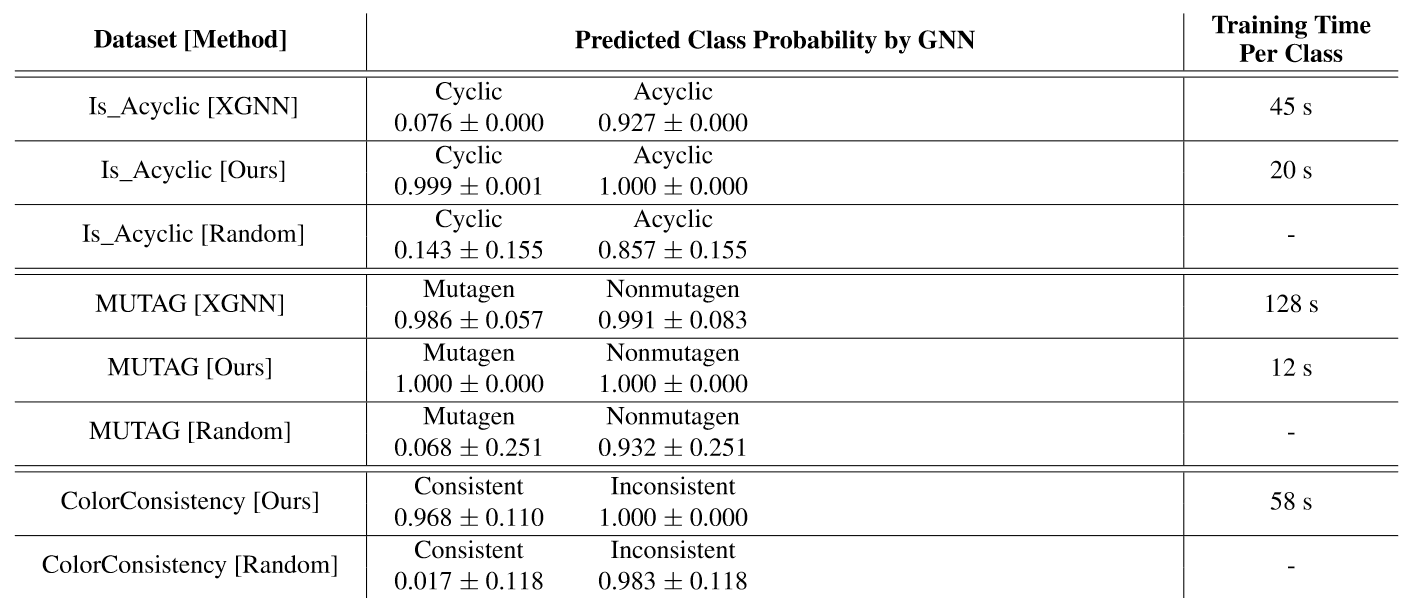
\includegraphics{figures/random_baseline.png} (X. Wang and Shen
    2024)
  \end{itemize}

  For example, random graphs have an average predicted probability of
  being Non-mutagenic in the MUTAG dataset if 93.2\%. This demonstrates
  why the above objective is insufficient to generate realistic or
  \emph{in-distribution} (id) graph.

  \begin{itemize}
  \tightlist
  \item
    In order to mitigate this issue, the author proposed additional
    minimizing the cosine distance between the average embedding of all
    the observed graph from the targeted class, \(\bar h^{(L)}_{G_c}\),
    and the embedding of the generated explanation.
  \end{itemize}

  \begin{equation}
       \mathcal{L}_{\text{embed}}(\Theta \ | \ G_\text{gen}) = 
            \mathams{E}_{G_\text{gen}}
            \text{CosDist}\left( \bar h^{(L)}_{G_c}, \ h^{(L)}_{G_\text{gen}} \right)
    \end{equation}
\item
  Regularization terms.

  \begin{itemize}
  \tightlist
  \item
    Sparse graphs are easy for humans to interpret. To encourage
    sparsity the authors employed an \(L_1\), \(L_2\), and a budget
    penalty on the edge probabilities.
  \end{itemize}

  \begin{equation}
        \mathcal{L}_{\text{Sparsity}}(\theta_A) = ||\theta_A||_1 + ||\theta_A||_2 + \text{softplus}(\text{sigmoid}||\theta_A||_1 - B)^2
    \end{equation} where \(B\) is the expected maximum number of edge
  for generated explanation graphs.

  \begin{itemize}
  \tightlist
  \item
    Connectivity is another desirable property as it ensures a cohesive
    explanation. To encourage connectivity the author minimize the
    \emph{KL-Divergence} between edge probabilities that share a common
    node.
  \end{itemize}

  \begin{equation}
        \mathcal{L}_{\text{Connect}}(\theta_A) = \sum_{i \in \nu} \sum_{j, k \in \mathcal{E}(i)} D_{KL}(\text{sigmoid}(\theta_A[i, \ j]) \ || \ \text{sigmoid}(\theta_A[i, \ k]))
    \end{equation}

  where \(\mathcal{E}(i)\) is the set of edges that connect to node
  \(i\).
\item
  Summary of Results + Figures

  \begin{itemize}
  \tightlist
  \item
    The final generator model is trained by sampling
    \(G_\text{gen} \sim \text{gen}(\Theta)\) and then iterative updated
    \(\Theta\) via gradient descent on the full loss: \begin{equation}
      \begin{split}
          \mathcal{L}_{\text{GNNInterpreter}}(\Theta \ | \ G_\text{gen}) = 
          &\mathcal{L}_{\text{pred}}(\Theta \ | \ G_\text{gen}) + 
          \mathcal{L}_{\text{embed}}(\Theta \ | \ G_\text{gen}) +  \\
          &\mathcal{L}_{\text{sparsity}}(\Theta \ | \ G_\text{gen}) +
          \mathcal{L}_{\text{connect}}(\Theta \ | \ G_\text{gen}) 
      \end{split}
      \end{equation}
  \end{itemize}

  \begin{figure}

  {\centering 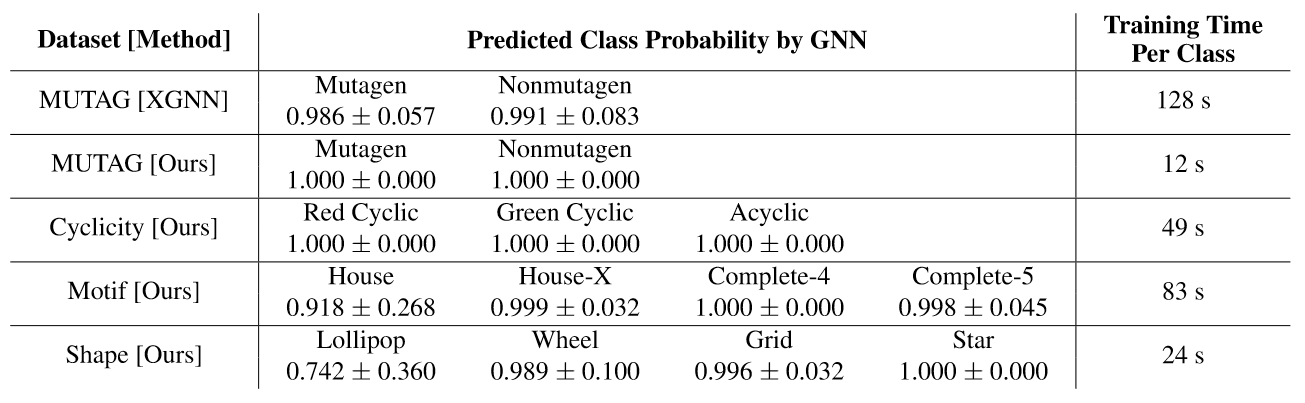
\includegraphics{figures/GNNInt_prediction_results.png}

  }

  \end{figure}

  \begin{itemize}
  \tightlist
  \item
    GNNInterpreter achieve remarkable accuracy on most target classes.
    Many of the interval are tight and very close to 1, which implies
    that the examples generated are almost always classified as the
    targeted class. The explanations for the house motif and the
    lollipop shape are worse in terms of predictions. Although the
    author critique the use of predictions as the sole objective, they
    do not use any other quantitative metric to evaluate the validity of
    their explanations.
  \end{itemize}

  \begin{figure}

  {\centering 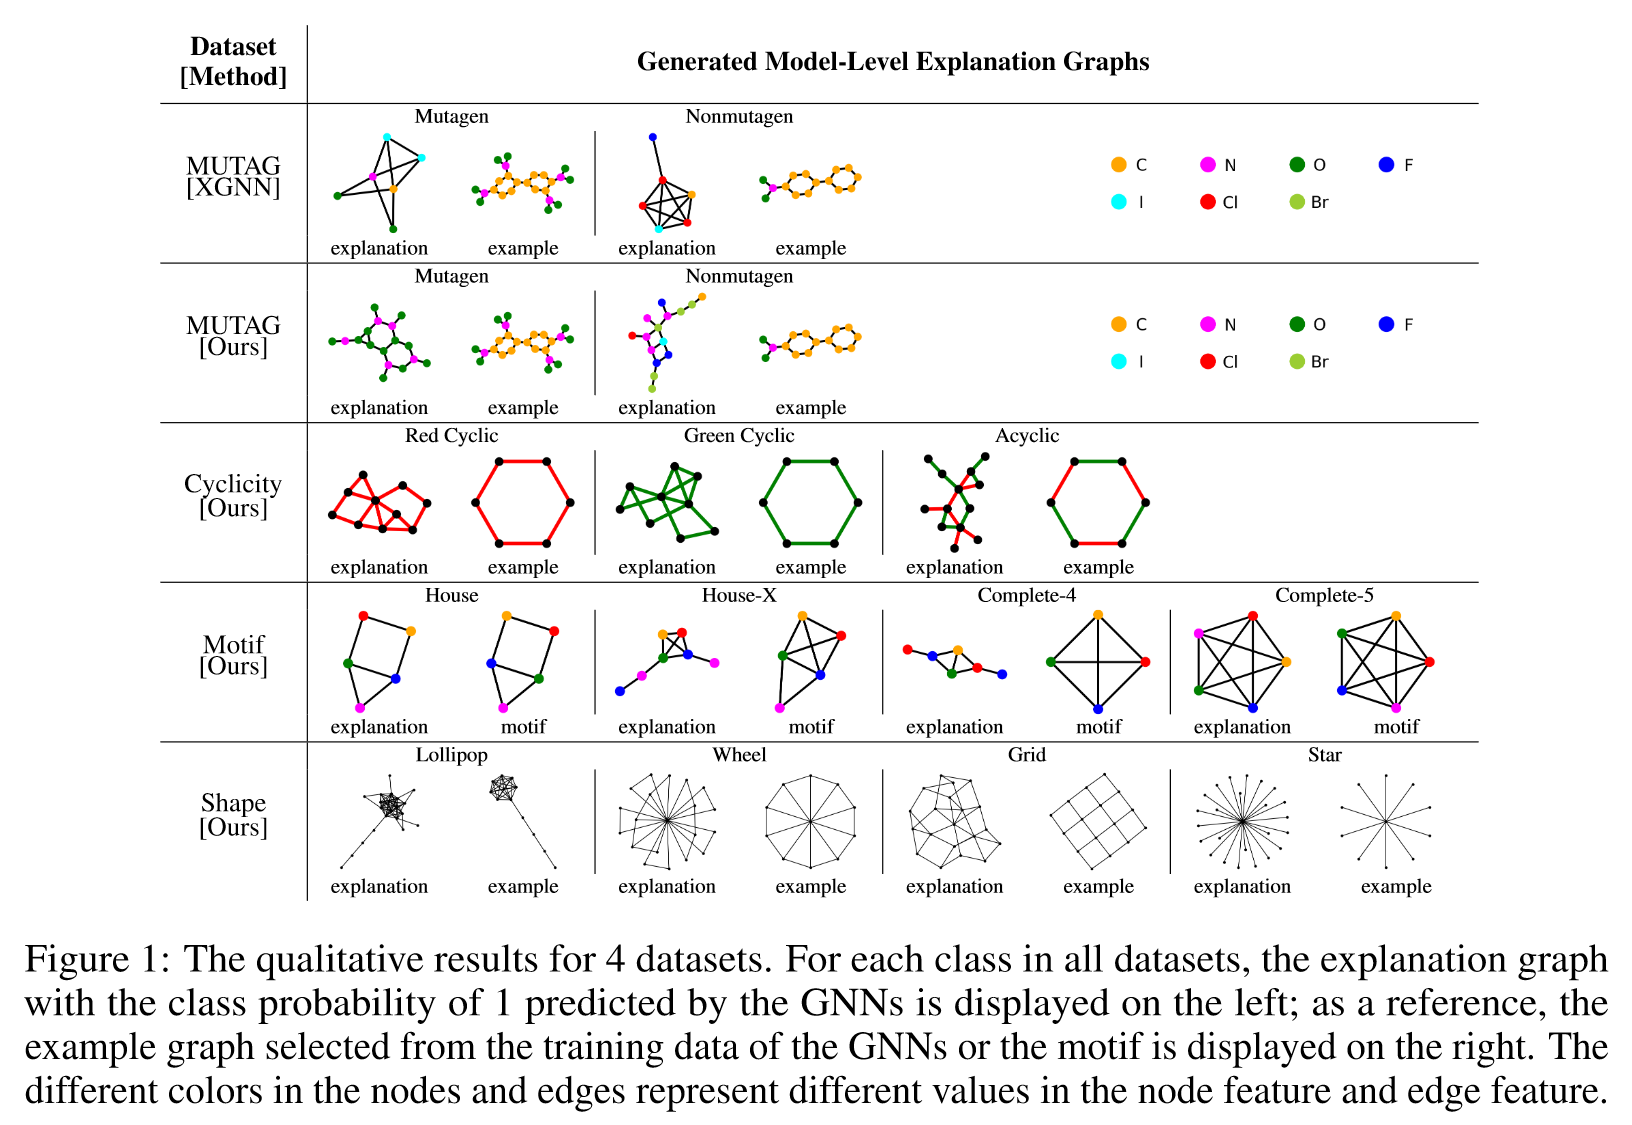
\includegraphics{figures/GNNInt_drawn_results.png}

  }

  \end{figure}

  \begin{itemize}
  \item
    Qualitatively we can see some limitation in terms of realism.
  \item
    For example, for the mutagen class, the explanation correctly
    identifies the importance of the N02 group; however, the generated
    graph isn't realistic and might not even be chemically possible.
    Furthermore, the non-mutagen example doesn't display any clear
    patterns or identifiable structures.
  \item
    The explanations for the Cyclicity dataset as well as the Wheel
    class do not appear to be members of the underlying data
    distribution.
  \item
    GNNInterpreter provides a way of generating example graph that would
    be classified as a target class by a GNN model, without needing to
    specify domain specific rules. On the other hand, optimizing
    predictions and even embeddings does not appear to be a sufficient
    objective for producing in-distribution graphs. The author correctly
    point out that optimizing predictions can lead to unrealistic
    graphs, but they have also inadvertently demonstrated that
    optimizing embeddings is not necessarily sufficient either.
  \end{itemize}
\end{itemize}

\hypertarget{d4explainer}{%
\subsection{D4Explainer}\label{d4explainer}}

(Chen et al. 2023)

\begin{itemize}
\item
  Overview

  \begin{itemize}
  \tightlist
  \item
    D4Explainer or in-Distribution GNN explanations via Discrete
    Denoising Diffusion attempt to directly address the realism of
    generated graphs in model-level explanation by using the observed
    data to train a Diffusion model.
  \item
    In the image domain, diffusion model have been shown to produce the
    most realistic images when compared to other generative AI methods
    such as Generative Adversarial Networks (GANs).
  \item
    Diffusion model work by iteratively noising an observation until it
    is pure noise. Then a denoising model is trained to predict the
    noise added at any given time step. Then new observations can be
    generated by passing pure noise through the diffusion model in a
    process known as reverse sampling.
  \item
    Additional label information can be passed to generate observations
    with similar a label.
  \end{itemize}
\item
  Forward Diffusion

  \begin{itemize}
  \item
    The authors here are focused on discrete structural diffusion.
    D4Explainer generate example graph by noising and de-nosing the
    adjacency matrices of observed graphs. The sampled graphs have the
    same features, but different structures.
  \item
    The process of gradually adding noise to the input data is called
    forward diffusion. During forward diffusion, random noise is added
    iteratively until the data becomes pure noise in the final
    iteration. This ensures that the denoising model can start with pure
    noise. Forward diffusion is usually a Markov process.
  \item
    If we assume that the observed graphs are Gilbert random graphs,
    like GNNInterpreter, pure noise would mean that
    \(\forall \ (i, \ j) \ A[i, j] \sim \text{Bernoulli(0.5)}\).
  \item
    Let \(t \in [0, T]\) denote the current iteration. Let \(\beta_t\)
    be the common probability that any edge changes state at time step
    \(t\). \((\beta_1, \dots, \beta_T)\) is known as the variance
    schedule and is a set hyperparameter. Let \(A_t\) be a one-hot
    encoded version of the \(t^{th}\) noised adjacency, \([1, 0]\) is
    the edge exists and \([0, 1]\) otherwise. Then the forward diffusion
    process can be expressed as:\\
    \begin{equation}
       A_t[i, j] \sim q(A_t[i, \ j] \ | \ A_{t-1}[i, \ j]) 
          = \text{Cat}(A_{t-1}[i, \ j] \cdot Q_t)
      \end{equation} or \begin{equation}
       A_t[i, j] \sim q(A_t[i, \ j] \ | \ A_{0}[i, \ j]) 
          = \text{Cat}\left(A_0[i, \ j] \prod_{i=1}^t  Q_i \right)
      \end{equation} where, \[
      Q_t = 
      \left[
      \begin{matrix}
      1-\beta_t & \beta_t \\ 
      \beta_t & 1 - \beta_t
      \end{matrix}
      \right]
      \] the \(t^{th}\) element-wise transition matrix.
  \item
    \textbf{Proof 2:}
    \(\lim_{t \to \infty} q(A_t[i, \ j] \ | \ A_{t-1}[i, \ j])  \overset{D}{\to}\)
    Bernoulli(0.5) (converges in distribution). \begin{align*}
       \lim_{t \to \infty} q(A_t[i, \ j] \ | \ A_{t-1}[i, \ j]) 
          &= \lim_{t \to \infty} \text{Cat}\left(A_0[i, \ j] \prod_{i=1}^t Q_i \right) \\
          &= \lim_{t \to \infty} \text{Cat}
          \left(A_0[i, \ j] 
              \prod_{i=1}^t  
              \left[
              \begin{matrix}
                  1  & -1 \\
                  1 & 1
              \end{matrix}
              \right]
              \left[
              \begin{matrix}
                  1  &  0 \\
                  0 & 1-2\beta_i
              \end{matrix}
              \right]
              \left[
              \begin{matrix}
                  0.5  &  0.5 \\
                  -0.5 & 0.5
              \end{matrix}
              \right]
          \right) \\ 
          &\text{Eigen decomposition.} \\ 
          &= \lim_{t \to \infty} \text{Cat}
          \left(A_0[i, \ j] 
              \left[
              \begin{matrix}
                  1  & -1 \\
                  1 & 1
              \end{matrix}
              \right]
              \left[
              \begin{matrix}
                  1  &  0 \\
                  0 & \prod_{i=1}^t 1-2\beta_i
              \end{matrix}
              \right]
              \left[
              \begin{matrix}
                  0.5  &  0.5 \\
                  -0.5 & 0.5
              \end{matrix}
              \right]
          \right) \\ 
          &= \text{Cat}
          \left(A_0[i, \ j] 
              \left[
              \begin{matrix}
                  1  & -1 \\
                  1 & 1
              \end{matrix}
              \right]
              \left[
              \begin{matrix}
                  1  &  0 \\
                  0 & 0
              \end{matrix}
              \right]
              \left[
              \begin{matrix}
                  0.5  &  0.5 \\
                  -0.5 & 0.5
              \end{matrix}
              \right]
          \right) \\ 
          &\text{Set }\beta < 0.5. \\
          &= \text{Cat}([0.5, 0.5]) = \text{Bernoulli}(0.5)
      \end{align*}
  \end{itemize}
\item
  Backward Diffusion (Denoising Model)

  \begin{itemize}
  \item
    A denoising model either predicts the error that was added or the
    value of the original observation. Even though only the adjacency
    matrix is being noised, we still want to include all available data.
    Thus the denoising model is parameterized as: \begin{equation}
       p(A_0 \ | \ A_t, t, X_0, E_0; \ \Omega)  
      \end{equation} where \(\Omega\) is the set of trainable
    parameters.
  \item
    The author employed a Provably Power Graph Network (PPGN) {[}cite{]}
    as their denoising model; however, they have added an additional
    neural network to learn the time or noise level effect.
  \end{itemize}
\item
  Loss Dist

  \begin{itemize}
  \tightlist
  \item
    Like most diffusion models, the primary objective is to minimize the
    distance between the predicted de-noised observation and the
    original. The author have added an additional weight term to focus
    the model on noisier or more difficult training examples.
    \begin{equation}
      \mathcal{L}_{dist} (\Omega \ | \ A_0) =  \sum_{t=1}^T 
          \left(1 - 2 \bar \beta_t + \dfrac 1 T \right)
          \mathams{E}_{\hat A_0}
          \text{CrtEnt} \left(
              A_0, \hat A_0
          \right)
      \end{equation} where
    \(\hat A_0 = p(A_0 \ | \ A_t, t, X_0, E_0; \ \hat \Omega)\),
    \(A_t[i, j] \sim q(A_t[i, \ j] \ | \ A_{0}[i, \ j])\), and \[
      \bar \beta_t = \frac 1 2 - \frac 1 2 \prod^t_{i=1}(1-2\beta_i)
      \] the cumulative transition probability.
  \end{itemize}
\item
  Model-level sampling algorithm

  \begin{itemize}
  \tightlist
  \item
    Use a set of observed graph features, D4Explainer generates model
    level explanations by sequentially denoising pure noise to generate
    an adjacency structure that has a high probability of being a member
    of the targeted class. At each step \(A_t\) is denoised to \(k\)
    candidates \(A_0, k\). The candidate with the best predicted
    probability is then noised to a level of \(t-1\) and the process is
    repeated. The pseudocode is reproduced below.
  \end{itemize}

  \begin{algorithm}
    \caption{D4Explainer Model-level Explanation Reverse Sampling Algorithm}\label{alg:cap}
    \begin{algorithmic}
        \Require $\hat \Omega$: trained denoising parameters; 
                $q(A_t \ | \ A_0)$: forward diffusion process.
        \renewcommand{\algorithmicrequire}{\textbf{Input:}}
        \renewcommand{\algorithmicensure}{\textbf{Output:}}
        \Require N: maximum number of nodes; T: maximum noise level; 
                K: number of candidates per iteration; 
                $\tilde{\rho}$ targeted prediction vector; 
                $(X, E)$: node and edge features.  
        \Ensure $\hat A$: adjacency matrix for model-level explanation.
        \State Sample $A_T[1:n, 1:n]$ \sim Bernoulli(0.5)
        \For{t in T to 1}
            \State Sample candidates 
                $\{\hat A_{0, k} \sim p(A_t,t, X, E; \ \hat \Omega) : k \in 1, \dots, K\}$
            \State Select the best candidate 
            $\underset{j \ \in \ i, \dots K}{\text{argmin}}$ 
            CrtEnt(explainee($G = (X, A_{0, j}, E)), \ \tilde{\rho}$)
            \State Sample $A_{t-1}[1:n, 1:n] \sim q(A_{t-1}, A_{0, j})$
        \EndFor
        \State \Return $A_0$
    \end{algorithmic}
    \end{algorithm}
\item
  In-Distribution metrics.

  \begin{itemize}
  \item
    To access how well a sampled explanation matches the observed graph
    distribution, the author compute various maximum mean discrepancy
    (mmd) statistics.
  \item
    MMD is a general technique to compute the distance between two
    distributions of data using only observed data. The distributions
    are estimated using a kernel an then the distance between there
    means are compared.
  \item
    A common way to approximate a density is to use the average of
    Gaussian distributions centered at each observation: \begin{align*}
      f(x)_X 
          &\approx \dfrac 1 n \dfrac{1}{\sqrt{2\pi}\sigma} 
          \sum_{i = 1}^n e^{\dfrac{-(x - x_i)^2}{2\sigma^2}} \\
          &\approx \dfrac 1 n \dfrac{1}{\sqrt{2\pi}\sigma} 
          \sum_{i = 1}^n \phi(x)^T \phi(x_i) 
      \end{align*} where, \(k(x_i, x_j) = \phi^T(x_i)^T \phi(x_j)\) is
    the Gaussian kernel function. As long as the chosen kernel is
    \emph{characteristic} the kernel mean embedding \[
      \dfrac 1 n \sum_{i = 1}^n \phi(x_i)^T = 
          \dfrac{1}{n} \phi(\vec{x}) \mathbb{1}
      \] is representative of the distribution. Here \(\vec x\) is the
    vector of observations and \(\mathbb{1}\) is the appropriate
    dimensional vector of 1s.
  \item
    MMD statistics are then simple the l2 distance between the kernel
    mean embeddings: \begin{align*}
       MMD(\vec x, \vec y) 
          &= 
          || 
          \dfrac{1}{n} \phi(\vec{x}) \mathbb{1} - 
          \dfrac{1}{m} \phi(\vec{y}) \mathbb{1}
          ||^2_2 \\
          &= 
          \left(
              \dfrac{1}{n} \phi(\vec{x}) \mathbb{1} -
              \dfrac{1}{m} \phi(\vec{y}) \mathbb{1}
          \right)^T
          \left(
              (\dfrac{1}{n} \phi(\vec{x}) \mathbb{1} -
              \dfrac{1}{m} \phi(\vec{y}) \mathbb{1}
          \right)^T \\
          &= 
          \dfrac{1}{n^2} \phi(\vec{x})^T \phi(\vec{x}) + 
          \dfrac{1}{m^2} \phi(\vec{y})^T \phi(\vec{y}) - 
          \dfrac{2}{nm} \phi(\vec{x})^T \phi(\vec{y})
      \end{align*}
  \item
    Intuitively \(\phi(\vec{x})^T \phi(\vec{x})\) and
    \(\phi(\vec{y})^T \phi(\vec{y})\) can be thought of as the distance
    within the observations of \(x\) and \(y\) and
    \(\phi(\vec{x})^T \phi(\vec{y})\) as the distance between. Therefore
    an MMD statistic close to zero means that the distribution are
    approximately the same.
  \item
    The author use MMD statistics to compare the degree, clustering, and
    spectrum distributions of the generated explanation against the
    observed data. The degree distribution of a graph indicates how
    frequently nodes have different numbers of connections, reflecting
    the overall connectivity pattern. The clustering coefficient of a
    node measures the proportion of the node's neighbors that are also
    connected to each other, representing local clustering. The spectrum
    distribution, which is the distribution of eigenvalues of the
    adjacency matrix or Laplacian matrix, provides insights into the
    graph's structural characteristics and dynamic properties.
  \item
    Like GNNInterpreter, the author of D4Explainer also value the
    sparsity of their generate example. They measure the density of a
    graph as the number of present edges divided by the number of
    possible edges or \begin{equation}
      \text{Density} = \mathcal{|E|} / |\nu|^2
      \end{equation}
  \end{itemize}
\item
  Loss CF

  \begin{itemize}
  \item
    In additional to model-level explanations, D4Explainer can provide
    \emph{counterfactual explanation} be include an additional term in
    the loss function. The authors define a counterfactual explanation
    for a particular observed graph to be \(G^c\) such that
    \(\hat Y_{G^c} \neq \hat Y_G\), but the difference between \(G^c\)
    and \(G\) is minimal.
  \item
    \(\mathcal{L}_{dist}\) ensures that the \(G^c\) generated won't
    deviate too far from the observed graph distribution.
  \item
    Adding \(\mathcal{L}_{CF}\) minimize the probability that the
    generated graph is classified the same as the input graph.
    \begin{equation}
       \mathcal{L}_{CF}(\Omega \ | \ A_0) = 
          \mathams{E}_{\hat A_0} - \log(1 - \rho_{G^c}[\hat Y_{G}])
      \end{equation} where \(G = (X, A, E)\) is an observed graph and
    \(G^c = (X, \hat A_0, E)\).
  \item
    To quantify the quality of generated counterfactual explanations,
    the author report \emph{Counterfactual Accuracy}, \emph{Fidelity},
    and modification ratio.

    \begin{itemize}
    \item
      CF-ACC measure the proportion of \(G^c\)s that have different
      predicted labels than there associated observed graph.\\
      \begin{equation}
         \text{CF-ACC} = \mathams{E}_{A_t} I(\hat Y_{G^c} \neq \hat Y_{G}) 
        \end{equation}
    \item
      Fidelity measures the difference in the predicted probability of
      \(G\) and \(G^c\) with respected to the original class label.\\
      \begin{equation}
        \text{Fidelity} = \mathams{E}_{\hat A_0} \rho_{G}[\hat Y_G] - \rho_{G^c}[\hat Y_G]
        \end{equation}
    \item
      Modification ratio measures difference in edges between \(G^c\)
      and \(G\) relative to the size of the original graph.\\
      \begin{equation}
        \text{MR} = \dfrac{|\sum_{i, j} A[i, j] - \hat A_0(i, j)|}{\sum_{i, j} A[i, j]}
        \end{equation}
    \end{itemize}
  \end{itemize}
\item
  Summary of Results + Figures

  \begin{itemize}
  \item
    Similar to GNNInterpreter, the author report the mean predicted
    probability for the targeted class. Using a maximum of 6 nodes, the
    author were able to achieve a mean of 0.832 on the MUTAG dataset.
  \item
    Since the counterfactual explanation are generated on a per
    observation basis, the author's compared their method to other
    popular instance-level explanation methods.
  \end{itemize}

  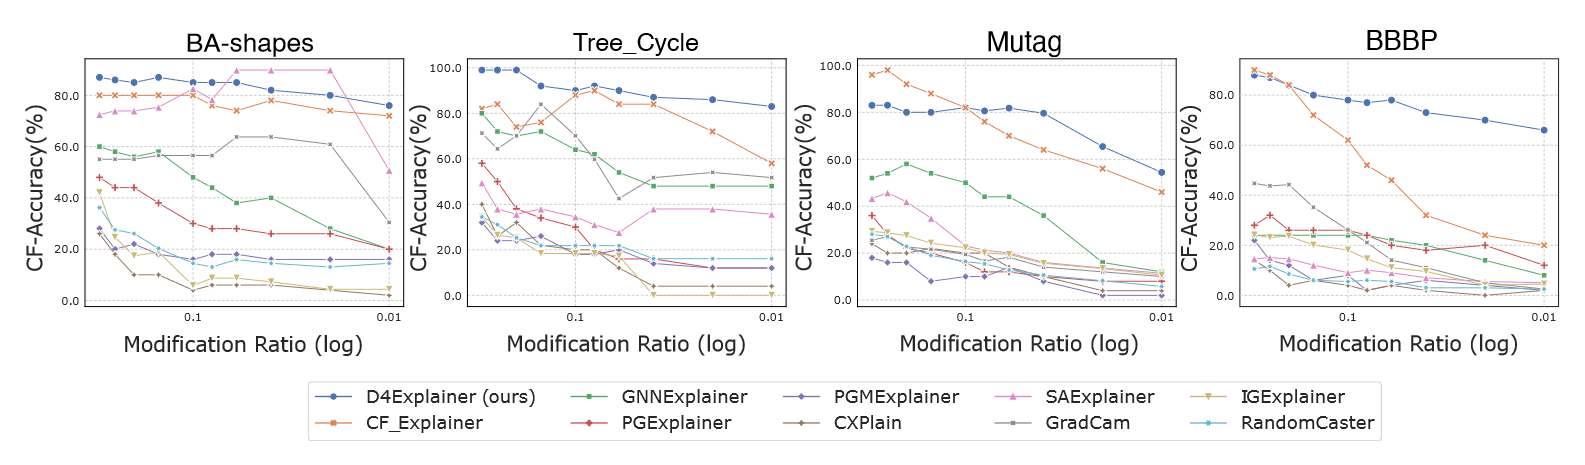
\includegraphics{figures/D4-CF-Plot.png} The above plot displays that
  D4Explainer can flip the prediction on \textasciitilde80\% of observed
  graphs at most modification levels. Missing from the plot is a
  variance measure. It is possible that the counterfactual accuracy
  varies more between different data splits or hyperparameter than the
  other methods.

  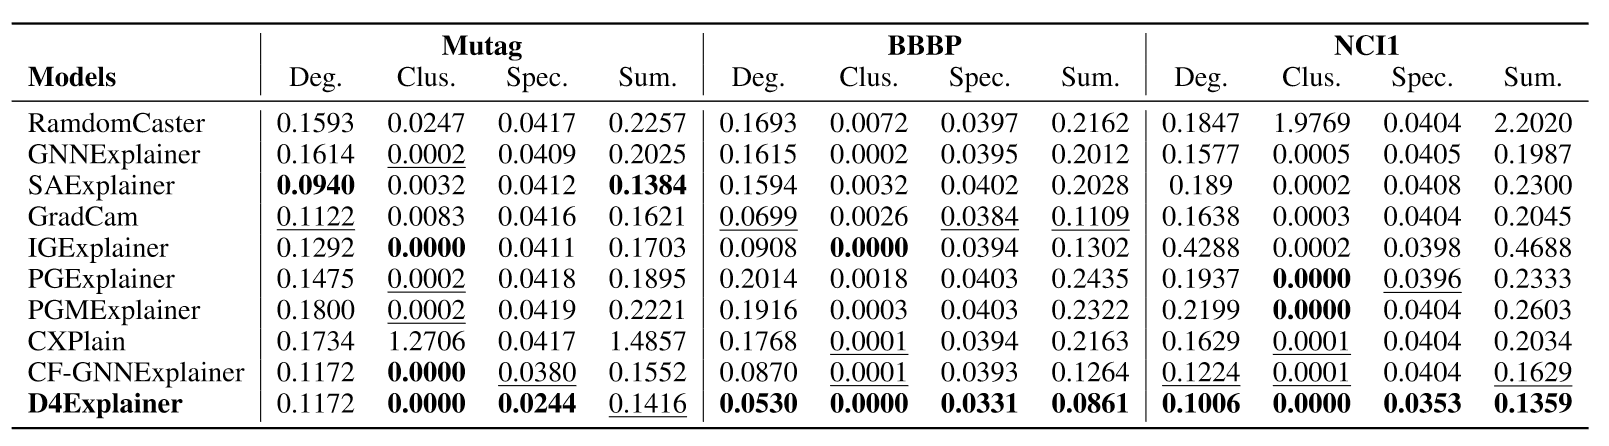
\includegraphics{figures/D4-MMD-Table.png} The above table indicates
  that the generated graph tend to have feature distribution that are
  close to the original dataset; however, there might be a hidden class
  bias. The distributions might only be close for the majority class,
  skewing the averages.
\end{itemize}

\hypertarget{protgnn}{%
\subsection{ProtGNN}\label{protgnn}}

(Zhang et al. 2021)

\hypertarget{synthesis-of-core-papers}{%
\section{Synthesis of Core Papers}\label{synthesis-of-core-papers}}

\begin{itemize}
\tightlist
\item
  Comparison of generation methods.

  \begin{itemize}
  \tightlist
  \item
    GNNInterpreter uses continuously relaxed discrete distributions.
  \item
    D4Explainer uses diffusion.
  \item
    Diffusion is slower, but can be more realistic. Probably because
    diffusion is less subject to the \textbf{out-of-distribution (OOD)
    problem}.
  \item
    Prototype projection are like generative methods. Restricted to in
    distribution, but realism is all but guaranteed.
  \end{itemize}
\end{itemize}

\hypertarget{technical-details}{%
\section{Technical Details}\label{technical-details}}

\hypertarget{methodology}{%
\subsection{Methodology}\label{methodology}}

\begin{itemize}
\item
  Since GNNInterpreter only makes qualitative assessments of generated
  structures, we applied the metrics describe in D4Explainer to quantify
  the properties of the generating distribution.
\item
  We reimplemented GNNInterpreter using an identical generation scheme
  and loss function.
\item
  We trained the reimplemented model on the MUTAG dataset which consists
  of nitroaromatic compounds, with the goal being to predict their
  mutagenicity on Salmonella typhimurium {[}cite{]}. Each observation is
  a graphs representing a chemical structure, where vertices denote
  atoms and edges represent bonds {[}cite{]}. MUTAG is a standard
  benchmark graph classification dataset.
\item
  For our explainee model, we also implemented a 3-layer GCN model.
  There are slight variations between the architectures and training
  hyperparameter, but the accuracies are comparable, 86\% (ours) and
  92\% (theirs).
\item
  We additionally reimplement D4Explainer's counterfactual generator.
  Although not discussed in the original paper, this model can also be
  used to produce model level explanations. We simply randomly sample a
  graph from the opposite class and take the generated counter factual
  graph as our explanation.
\end{itemize}

\hypertarget{results}{%
\subsection{Results}\label{results}}

\begin{longtable}[t]{llllll}
\caption{}\\
\toprule
  & Predictions & Density & Deg. & Clus. & Spec.\\
\midrule
\addlinespace[0.3em]
\multicolumn{6}{l}{\textbf{GNNInterpreter Original}}\\
\hspace{1em}Class 0 & 1.0 +/- 0.0 & NA & NA & NA & NA\\
\hspace{1em}Class 1 & 1.0 +/- 0.0 & NA & NA & NA & NA\\
\addlinespace[0.3em]
\multicolumn{6}{l}{\textbf{GNNInterpreter Reimplemented}}\\
\hspace{1em}Class 0 & 0.93 +/- 0.01 & 0.38 +/- 0.002 & 1.77 & 1.53 & 0.07\\
\hspace{1em}Class 1 & 0.98 +/- 0.01 & 0.32 +/- 0.003 & 1.41 & 1.43 & 0.04\\
\addlinespace[0.3em]
\multicolumn{6}{l}{\textbf{D4Explainer Original}}\\
\hspace{1em}Aggregated & 0.92 & 0.315 & 0.12 & 0.00 & 0.02\\
\addlinespace[0.3em]
\multicolumn{6}{l}{\textbf{D4Explainer Reimplemented}}\\
\hspace{1em}Class 0 & 0.63 +/- 0.23 & 0.13 +/- 0.03 & 0.27 & 0.57 & 0.05\\
\hspace{1em}Class 1 & 0.66 +/- 0.20 & 0.13 +/- 0.03 & 0.08 & 0.25 & 0.04\\
\bottomrule
\multicolumn{6}{l}{\rule{0pt}{1em}\textsuperscript{1} +/- 1 standard deviation; 1000 graphs.}\\
\multicolumn{6}{l}{\rule{0pt}{1em}\textsuperscript{*} Empty}\\
\end{longtable}

\begin{figure}

{\centering 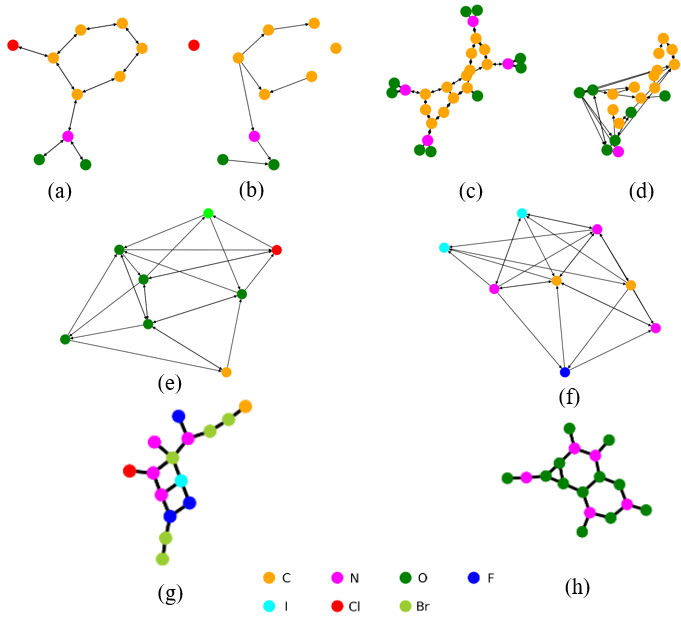
\includegraphics[width=0.8\textwidth,height=0.8\textheight]{figures/mutag_plot_together.png}

}

\caption{(a) Observed graph from class 0, Pr = 0.92; (b) Generated
counterfactual explanation of (a) from D4Explainer reimplemented, Pr =
0.67; (c) Observed graph from class 1, Pr = 0.96; (d) Generated
counterfactual explanation of (b) from D4Explainer reimplemented, Pr =
0.96; (e) Generated explanation for class 0 from GNNInterpreter
reimplemented, Pr = 0.94; (f) Generated explanation for class 1 from
GNNInterpreter reimplemented, Pr = 1.0; (g) Generated explanation for
class 0 from GNNInterpreter (Wang and Shen 2024, fig.~1, pg.7), Pr =
1.0; (h) Generated explanation for class 1 from GNNInterpreter (Wang and
Shen 2024, fig.~1, pg.7), Pr = 1.0.}

\end{figure}

\begin{itemize}
\item
  We were unable to achieve 0 variance predictive accuracy, but again
  the values are comparable (see table ?) given the lack of extensive
  hyperparameter tuning. The prediction are similarity superior to that
  of D4Explainer (see table ?).
\item
  As noted by the authors, the explainee model has a bias towards the
  mutagenic class (class 0), which can explain the greater deviation
  between the class 0 models.
\item
  Another limiting factor is a lower set maximum number of nodes. We set
  it to 8 to make the results more comparable to the model-level
  explanation reported by D4Explainer.
\item
  Surprisingly D4Explainer produces sparser graphs, in terms of density,
  than GNNInterpreter, despite no explicit penalty in the loss function.
\item
  Based on the MMD statistics, the D4Explainer produces graph with
  better in-distribution properties. This might be the result of the
  explicit regularization in GNNInterpreter. Penalize the edge
  probabilities should result in a different degree distribution. The
  clustering coefficient might also be effect since fewer edges result
  in fewer triangle clusters.
\item
  The spectrum distributions are close for both model, since both model
  enforce similarity in the explainee embedding space which is similar
  to the nature of the spectrum distribution.
\item
  On the other hand, an argument could be made that a similar degree
  distribution and clustering coefficient isn't actually desirable. For
  larger or more densely connected graphs, lower MMD statistics might
  results in explanations that are too complex to be useful.
\item
  Similar to the original examples display in GNNInterpreter, the
  generated non-mutagenic graphs do not have clear or realistic
  structures. Graph (f) highlights that nitrogen in key. We believe that
  this result is consistent with the original findings about the N02
  groups, but because of the more restrictive node limit, our
  reproduction focuses on nitrogen since multiple oxygens can be found
  in non-mutagenic chemicals.
\item
  The reimplement D4Explainer has a CF-ACC in line with the original
  paper, 76.32\% at 0.41 log MR.
\item
  The reimplement D4Explainer produces the least dense graphs, but has
  the least discriminative predictions. The latter makes sense, since
  the goal of the counterfactual loss is to flip the prediction, not
  necessarily maximize it.
\item
  One the other hand, this model demonstrates that it is possible to
  generate sparse predictions and maintain a similar degree distribution
  and clustering.
\item
  Visually the counterfactual explanation make sense. Graph (b)
  eliminated the red or chlorine atom which is typically associated with
  non-mutagenic compounds {[}XGNN{]}. Graph (d) corrupted 3 of the 4 N02
  groups, which is in line with GNNInterpreter's findings that multiple
  N02 groups is a strong indicator of mutagenicity.
\item
  This results lead to two main conclusions.

  \begin{itemize}
  \item
    First, the generator model should make use of the graph level
    observations. GNNInterpreter only use information about the graph
    structure through the explainee, never on the raw scale.

    \begin{itemize}
    \item
      This lack of graph level information result can result in
      unrealistic distributional properties.
    \item
      This could be done by using the observed graphs to predict the
      distributional parameters.
    \item
      Alternatively, the generator could be replaced with a diffusion
      model without any need to modify the loss.
    \end{itemize}
  \item
    Second, the generator model should use class or prediction
    information.

    \begin{itemize}
    \item
      D4Explainer's model-level sampling algorithm is less efficient and
      less accuracy than GNNInterpreter's direct optimization during
      training.
    \item
      The reimplemented sampling algorithm demonstrates that direct
      denoising can still maintain low MMD statistics.
    \item
      A possible modification would be to add the
      \(\mathcal{L}_\text{pred}\) and \(\mathcal{L}_\text{embed}\) from
      GNNInterpreter to the loss.
    \item
      Alternatively, one could embedding the class label, similar to the
      way time is embedded, in order to establish a conditional
      diffusion model, which has worked extremely well in other
      applications.
    \item
      Additionally, it would be easy to explore diffusing the node and
      edge features as well as like \emph{DiGress} {[}cite{]}.
    \end{itemize}
  \end{itemize}
\end{itemize}

\hypertarget{future-directions}{%
\section{Future Directions}\label{future-directions}}

\hypertarget{graph-edit-distance}{%
\subsection{Graph Edit Distance}\label{graph-edit-distance}}

\begin{itemize}
\item
  GNNInterpreter generates graphs with predictions very close to the
  target class, but lack good in-distributions properties.
\item
  D4Explainer generates explanations with more similar features
  distributions to the observed data; however, the predicted
  probabilities show more variance. Furthermore, while the model
  parameters of GNNInterpreter's generator can be interpreted,
  D4Explainer introduces another black-box model.
\item
  We propose using a differentiable approximation to the graph edit
  distance as a way of generically enforcing structural consistency.
\item
  GED measures the similarity between two graphs by counting the minimum
  number of edits required to make the graphs isomorphic (or subgraph
  isomorphic). Similar to the modification ratio for counterfactual
  explanations.
\item
  This has the key advantage of being human interpretable. For example,
  the percentage of atoms and bonds that need to be changed for two
  molecules to match is more relatable than the cosine distance between
  their embeddings.
\item
  Finding the exact optimal GED is a known NP-complete problem, and most
  solutions are not differentiable (Bougleux et al. 2015).
\item
  Fortunately, approximating GED as a quadratic assignment problem (QAP)
  solves both the time complexity and derivative issue (R. Wang et al.
  2024).
\end{itemize}

Let \(G_1\) and \(G_2\) be graphs we wish to compute the GED between.
QAP approximates this be solving the following optimization problem:
\begin{equation}
    \mathcal{L}_{\text{GED}} = \underset{M}{\max} \ \text{vec}(M) \ K(G_1, G_2) \ \text{vec}(M)^T
\end{equation} here \(M\) is a \((n_1 \times n_2)\) binary node matching
matrix and \(K\) is a \((n_1 n_2 \times n_1 n_2)\) quadratic affinity
matrix that encode both node and edge similarity information. The
efficiency of QAP comes from the fact that when any two nodes are
matched together, the above objective will account for the possible
edges that could connect the nodes. In order to compute GED, each entry
of \(K\) should range from {[}-1, 0{]}, where -1 signals the need for a
complete edit and 0 means no edits are required (R. Wang et al. 2024).
We use the following similarity metric for every pair of nodes and
edges: \begin{equation}
    \begin{split}
         &-0.25 \left[ 1 - \phi(\text{Continuous Features}) \right] \ + \\
         &-0.5 \left[1 - \phi(\text{Discrete Features}) \right]
    \end{split}
\end{equation} where \(\phi(.)\) is the normalized cosine distance.
\(1 - \phi(.)\) will return 2 is the vectors are in opposite directions,
1 if the vectors are orthogonal, and 0 if they are pointing in the same
direction; however, one-hot encoded vectors will never be in opposite
directions, so the different types of feature must be weighted
correctly. Computing affinity this way allows for \(K\) to be
differentiable w.r.t. generated graph features. Furthermore we use the
reweighted random walks algorithm (Cho, Lee, and Lee 2010) to solve the
above objective, which generates an M that is differentiable w.r.t. to
K.

\begin{itemize}
\item
  We conducted a simulation study to compare graph level and latent
  similarity, or \(\mathcal{L}_{\text{GED}}\) and
  \(\mathcal{L}_{\text{embed}}\).
\item
  We generated 4 clusters of graph data. Every graph had one continuous
  edge feature sampled from a standard normal, one discrete node and
  edge feature sampled from a Bernoulli, and an adjacency matrix also
  Bernoulli. The only variation between the clusters was the maximum
  number of nodes as well as the mean of the continuous node feature
  distribution. Cluster 0 had 75-100 nodes, cluster 1 had 50-75 nodes,
  and cluster 2 as well as 3 had 10-35 nodes. This was designed to mimic
  a classic binary graph classification dataset where cluster 0 and 1
  are the observed classes and clusters 2 and 3 are generated subgraph
  explanations. The embedding model was a 3 layer graph convolution
  network with a neural network type convolution that utilized every
  feature.
\item
  During each of the 50 trials, the GCN was trained using 50 samples
  (each) from only clusters 0 and 1. We then sampled 50 test graphs from
  each of the 4 cluster and computed 95\% t intervals for GED and
  embedding cosine distance as percentages of their respective upper
  bounds. Since \((\mu_0 = -1, \mu_1 = 1, \mu_2 = 0, \mu_3 = -5)\) we
  would expect an unbiased distance metric to maintain the following
  relationship, \begin{equation}
    \text{dist}(1,\ 2) \approx \text{dist}(0, 2) < \text{dist}(0, 1) < \text{dist}(0, 3) < \text{dist}(1, 3)
  \end{equation} based on the distance between cluster means.
\end{itemize}

\begin{longtable}[t]{lcc}
\caption{Simulation Results}\\
\toprule
  & Cluster 0 & Cluster 1\\
\midrule
\addlinespace[0.3em]
\multicolumn{3}{l}{\textbf{Embeddings}}\\
\hspace{1em}Within & (0.0008, 0.0015) & (0.0005, 0.0009)\\
\hspace{1em}Between & (0.5662, 0.6264) & (0.5689, 0.6289)\\
\hspace{1em}Cluster 2 & (0.2894, 0.3589) & (0.1282, 0.209)\\
\hspace{1em}Cluster 3 & (0.018, 0.0253) & (0.6521, 0.7097)\\
\addlinespace[0.3em]
\multicolumn{3}{l}{\textbf{GED}}\\
\hspace{1em}Within & (0.4147, 0.419) & (0.462, 0.4674)\\
\hspace{1em}Between & (0.6589, 0.6639) & (0.6586, 0.6646)\\
\hspace{1em}Cluster 2 & (0.7843, 0.7947) & (0.7571, 0.7715)\\
\hspace{1em}Cluster 3 & (0.6164, 0.6286) & (0.8256, 0.8352)\\
\bottomrule
\multicolumn{3}{l}{\rule{0pt}{1em}\textsuperscript{1} Node Means: $\mu_0 = -1$, $\mu_1 = 1$, $\mu_{out1} = 0$, 
                    $\mu_{out2}$ = -5.}\\
\multicolumn{3}{l}{\rule{0pt}{1em}\textsuperscript{2} 95\% t intervals on \% difference.}\\
\end{longtable}

\begin{align*}
    \text{Expected: } &\text{dist}(1,\ 2) \approx \text{dist}(0, 2) < \text{dist}(0, 1) < \\ 
    &\text{dist}(0, 3) < \text{dist}(1, 3) \\ 
    \text{GED: }&(0.75, 0.77) \textcolor{green}{\approx} (0.78, 0.79) 
                \textcolor{red}{>} (0.65, 0.66) \textcolor{red}{>} \\
                &(0.61, 0.62) \textcolor{green}{<} (0.82, 0.83) \\
    \text{Embedding: }&(0.12, 0.20) \textcolor{red}{<} (0.28, 0.35) 
                \textcolor{green}{<} (0.56, 0.62) \textcolor{red}{>>} \\
                &(0.018, 0.0253) \textcolor{green}{<} (0.65, 0.7)
\end{align*} The most worrisome bias arises between the distances from
cluster 0 to 1 and from cluster 0 to 3. Despite cluster 0's mean being
twice as close to cluster 1, the embedding distance indicates that
cluster 0 is (53, 60) percentage points farther away from cluster 1.
Although GED also displayed this bias, it was considerably less
pronounced, registering at (1, 5) percentage points. This implies that a
generator initialized with a mean of -5 would produce samples with
embeddings confidently assigning them to cluster 0, despite having a
feature distribution far from the truth. Relying solely on embedding
distance for training also increases the likelihood of the generator
becoming trapped in a misleading local optimum due to the substantial
bias. Although GED exhibits a statistically significant bias, its
magnitude is considerably smaller, making it less likely to disrupt
training. Another troubling bias observed is that the embedding distance
between clusters 1 and 2 is approximately 10 percentage points less than
the embedding distance between clusters 0 and 2, even though the mean of
cluster 2 is equidistant from the means of clusters 1 and 0. This could
stem from cluster 1 having fewer nodes making samples more similar in
terms of size to cluster 2. However, since researcher typically cap the
size of examples for interpretability, an objective with a degree bias
could be problematic. On the contrary, GED introduces a bias absent in
the embedding space. The edit distance between clusters 0 and 2 is
actually greater than the distance between clusters 0 and 1. While
biased concerning mean locations, this direction is aligned with the
maximum node size. Despite this, the differing directions of the biases
of GED and embedding distance imply that they capture unique structural
nuances, potentially complementing each other.

\begin{itemize}
\tightlist
\item
  \(\mathcal{L}_{\text{GED}}\) could also be added to the loss function
  for D4Explainer as well.
\end{itemize}

\hypertarget{graph-prototype-masking-network}{%
\subsection{Graph Prototype Masking
Network}\label{graph-prototype-masking-network}}

\begin{itemize}
\item
  Theory
\item
  Diagram
\end{itemize}

\pagebreak

\hypertarget{references}{%
\section*{References}\label{references}}
\addcontentsline{toc}{section}{References}

\hypertarget{refs}{}
\begin{CSLReferences}{1}{0}
\leavevmode\vadjust pre{\hypertarget{ref-bai2019unsupervised}{}}%
Bai, Yunsheng, Hao Ding, Yang Qiao, Agustin Marinovic, Ken Gu, Ting
Chen, Yizhou Sun, and Wei Wang. 2019. {``Unsupervised Inductive
Graph-Level Representation Learning via Graph-Graph Proximity.''}
\url{https://arxiv.org/abs/1904.01098}.

\leavevmode\vadjust pre{\hypertarget{ref-Bougleux_Brun_Carletti_Foggia_Gauxfczuxe8re_Vento_2015}{}}%
Bougleux, Sébastien, Luc Brun, Vincenzo Carletti, Pasquale Foggia,
Benoit Gaüzère, and Mario Vento. 2015. {``A Quadratic Assignment
Formulation of the Graph Edit Distance,''} no. arXiv:1512.07494
(December). \url{http://arxiv.org/abs/1512.07494}.

\leavevmode\vadjust pre{\hypertarget{ref-Chen_Wu_Gupta_Ying_2023}{}}%
Chen, Jialin, Shirley Wu, Abhijit Gupta, and Rex Ying. 2023.
{``D4Explainer: In-Distribution GNN Explanations via Discrete Denoising
Diffusion,''} no. arXiv:2310.19321 (October).
\url{https://doi.org/10.48550/arXiv.2310.19321}.

\leavevmode\vadjust pre{\hypertarget{ref-Cho_Lee_Lee_2010}{}}%
Cho, Minsu, Jungmin Lee, and Kyoung Mu Lee. 2010. {``Reweighted Random
Walks for Graph Matching.''} In \emph{Computer Vision -- ECCV 2010},
edited by Kostas Daniilidis, Petros Maragos, and Nikos Paragios,
492--505. Lecture Notes in Computer Science. Berlin, Heidelberg:
Springer. \url{https://doi.org/10.1007/978-3-642-15555-0_36}.

\leavevmode\vadjust pre{\hypertarget{ref-gallicchio2019fast}{}}%
Gallicchio, Claudio, and Alessio Micheli. 2019. {``Fast and Deep Graph
Neural Networks.''} \url{https://arxiv.org/abs/1911.08941}.

\leavevmode\vadjust pre{\hypertarget{ref-Huijben_Kool_Paulus_van_Sloun_2022}{}}%
Huijben, Iris A. M., Wouter Kool, Max B. Paulus, and Ruud J. G. van
Sloun. 2022. {``A Review of the Gumbel-Max Trick and Its Extensions for
Discrete Stochasticity in Machine Learning,''} no. arXiv:2110.01515
(March). \url{https://doi.org/10.48550/arXiv.2110.01515}.

\leavevmode\vadjust pre{\hypertarget{ref-Maddison_Mnih_Teh_2017}{}}%
Maddison, Chris J., Andriy Mnih, and Yee Whye Teh. 2017. {``The Concrete
Distribution: A Continuous Relaxation of Discrete Random Variables,''}
no. arXiv:1611.00712 (March).
\url{https://doi.org/10.48550/arXiv.1611.00712}.

\leavevmode\vadjust pre{\hypertarget{ref-wang2024pygm}{}}%
Wang, Runzhong, Ziao Guo, Wenzheng Pan, Jiale Ma, Yikai Zhang, Nan Yang,
Qi Liu, et al. 2024. {``Pygmtools: A Python Graph Matching Toolkit.''}
\emph{Journal of Machine Learning Research} 25 (33): 1--7.
\url{https://jmlr.org/papers/v25/23-0572.html}.

\leavevmode\vadjust pre{\hypertarget{ref-Wang_Shen_2024}{}}%
Wang, Xiaoqi, and Han-Wei Shen. 2024. {``GNNInterpreter: A Probabilistic
Generative Model-Level Explanation for Graph Neural Networks,''} no.
arXiv:2209.07924 (February).
\url{https://doi.org/10.48550/arXiv.2209.07924}.

\leavevmode\vadjust pre{\hypertarget{ref-Xiao_Wang_Rong_Yang_Zhang_Zhan_Bishop_Wilhelm_Zhang_Pickering_et_al._2023}{}}%
Xiao, Guanghua, Shidan Wang, Ruichen Rong, Donghan Yang, Xinyi Zhang,
Xiaowei Zhan, Justin Bishop, et al. 2023. \emph{Deep Learning of Cell
Spatial Organizations Identifies Clinically Relevant Insights in Tissue
Images}. Preprint. In Review.
\url{https://doi.org/10.21203/rs.3.rs-2928838/v1}.

\leavevmode\vadjust pre{\hypertarget{ref-Yuan_Yu_Gui_Ji_2022}{}}%
Yuan, Hao, Haiyang Yu, Shurui Gui, and Shuiwang Ji. 2022.
{``Explainability in Graph Neural Networks: A Taxonomic Survey,''} no.
arXiv:2012.15445 (July).
\url{https://doi.org/10.48550/arXiv.2012.15445}.

\leavevmode\vadjust pre{\hypertarget{ref-Zhang_Liu_Wang_Lu_Lee_2021}{}}%
Zhang, Zaixi, Qi Liu, Hao Wang, Chengqiang Lu, and Cheekong Lee. 2021.
{``ProtGNN: Towards Self-Explaining Graph Neural Networks,''} no.
arXiv:2112.00911 (December).
\url{https://doi.org/10.48550/arXiv.2112.00911}.

\end{CSLReferences}



\end{document}
